\documentclass[a4paper,12pt,  twoside, openright,final]{memoir}


% INPUT PACKAGES %
\usepackage[utf8]{inputenc}						% INPUT FORMATERING SOM SIKRE AT VI KAN SKRIVE Æ,Ø og Å
\usepackage[british, danish]{babel}						% PÅBEGYNDER DANSK ORDDELING
\renewcommand{\danishhyphenmins}{22}				% BEDRE DANSK ORDDELING
\usepackage[T1]{fontenc}						% PÆNERE DANSK FONT ENKODNING
%\usepackage{fontspec}							% Special fonts
%\setmainfont{Arial} 							% Sæt skrift typen til Source Sans Pro

% ASSISTING PACKAGES %
\usepackage{hyperref}
\hypersetup{
	colorlinks = true,
	citecolor = blue}
\usepackage[nopar]{lipsum}						% GENERER FYLDTEKST
\usepackage{showkeys}							% SHOWS THE LABELS OF FIGURES, TABLES, ETC...
\usepackage{graphicx}							% DISPLAY GRAPHICS ETC.
\usepackage{smartdiagram}						% NEMMEDIAGRAMMER
\usepackage[natbibapa]{apacite}					% APACITE AND NATBIB
\bibliographystyle{apacite}						% ACTIVATE APACITE
\usepackage[danish]{varioref}						% VARIATIONS IN REFERENCES
\usepackage{fixme}
\usepackage{soul}								% Huphenable letterspacing
\usepackage{xcolor}
\usepackage{wrapfig}
%\usepackage{paperandpencil}						% Spørgeskema pakke
%\usepackage[lines=40, chars=60,noindent]{stdpage}

\sodef\an{}{0.2em}{0.9em plus 0.6 em}{1em plus .1em minus .1em}
\newcommand\stext[1]{\an{\scshape#1}}

% PAGE SETUP REMARKS %
\setlrmarginsandblock{*}{3.5cm}{0.75}					% HØJRE OG VENSTRE
\setulmarginsandblock{3cm}{*}{1.2}					% TOP OG BUND
\checkandfixthelayout[nearest]						% SPECIFIKT VALG AF HØJDE ALGORITME

% STYLING THE CHAPTER %
\definecolor{TMA}{rgb}{.255,.102,0}
\renewcommand\colorchapnum{\color{TMA}}
\renewcommand\colorchaptitle{\color{TMA}}
\chapterstyle{madsen}

% PAGE HEADER AND FOOTER %
\makepagestyle {TMArules}
\makeheadrule   {TMArules}{\textwidth}{\normalrulethickness}
\makefootrule    {TMArules}{\textwidth}{\normalrulethickness}{\footruleskip}
\makeevenhead {TMArules}{}{}{\small\itshape\leftmark}
\makeoddhead   {TMArules}{\small\itshape\rightmark}{}{}
\makeevenfoot   {TMArules}{}{}{\small \bfseries\thepage}
\makeoddfoot    {TMArules}{\small \bfseries\thepage} {}{}
\makeatletter % because of \"chapapp
\makepsmarks {TMArules}{
\nouppercaseheads
\createmark {chapter} {both} {shownumber}{\@chapapp\ }{. \ }
\createmark {section} {right}{shownumber}{} {. \ }
\createmark {subsection} {right}{shownumber}{} {. \ }
\createmark {subsubsection}{right}{shownumber}{} {. \ }
\createplainmark {toc} {both} {\contentsname}
\createplainmark {lof} {both} {\listfigurename}
\createplainmark {lot} {both} {\listtablename}
\createplainmark {bib} {both} {\bibname}
\createplainmark {index} {both} {\indexname}
\createplainmark {glossary} {both} {\glossaryname}
}
\makeatother
\setsecnumdepth{subsubsection}
\pagestyle{TMArules}


% APPENDIX CUSTOMISATION %
\addto\captionsdanish{\renewcommand\appendixname{Bilag}}
\DeclareRobustCommand{\changetoapp}{%
	\renewcommand*{\cftchapterpresnum}{\appendixname\space}%
	\setlength{\cftchapternumwidth}{7em}
}
\let\oldappendix\appendix
\renewcommand*{\appendix}{\oldappendix
	\addtocontents{toc}{\changetoapp}}

\title{Test dokument\ldots}
\author{Thomas M. Amby}



% ------------------------ INCLUDE LIST ----------------------- %
\includeonly{Afsnit/Kapitel1, Afsnit/Kapitel2}

\begin{document}
\begin{titlingpage}
	\thispagestyle{empty}
	\centering
	{
		\setlength{\baselineskip}{24pt}
		{
			\Huge \stext{UndersøgelsesBaseret NaturfagsUndervisning} \par
			\textit{\&} \par
			\stext{Science Writing Heuristic}
		}\par
		\stext{(Om skriftlighed i fysikfaget ved det almene gymnasium)}
		\par\vspace*{4\onelineskip}
		\par
		
\includegraphics[width=\textwidth]{Figs/Pen}
		\par\vspace*{4\onelineskip}
		\stext{Master projekt i Science Undervisning}\par
		\large\stext{Thomas Mellergaard Amby --- 20051837}\par
	}
	\vfill
	\vspace*{2\onelineskip}
	\stext{Vejleder: Jesper Bruun}\hfill
	\stext{6. Maj 2019}
	\par\vspace*{2\onelineskip}
	\small
	\stext{Institut for Naturfagenes Didaktik}\par
	\stext{Københavns Universitet \& Aarhus Universitet}
	\enlargethispage{2\onelineskip}
\end{titlingpage}
%\maketitle

% --------- FRONTMATTER --------- %
\frontmatter
\begin{otherlanguage}{british}
	\begin{abstract}
		This the English abstract\ldots
	\end{abstract}
\end{otherlanguage}
\clearpage
\tableofcontents

% -------- MAINMATTER -----------%
 \mainmatter


\chapter{Introduktion}
\label{Ch:1}

Denne opgave beskæftiger sig med elevernes skriftlige arbejde i fysik faget, herunder undersøges elevernes motivation i forhold til både det praktiske arbejde og til det skriftlige arbejde med faget. Den praktiske dimension af de naturvidenskabelige fag har tidligere været et adelsmærke for hvordan fagene tænkes at kunne motivere eleverne. Studier som fx \citep{Hodson2008} peger på at man måske overfortolker betydningen af det praktiske arbejde som motivation for eleverne. Det er interessant at undersøge sammenhængen mellem det praktiske arbejde og elevernes motivation for faget og for skriftligheden, i en dansk kontekst, da \citep{Hodson2008} ikke inddrager danske data. Alle de studier som forelægger på nuværende tidspunkt omhandler enten elever i grundskolen eller studerende på universitet. Der foreligger ingen studier som er udført i en dansk undervisnings kontekst. Derfor er det interessant at undersøge hvorledes man kan påvirke elevernes læring ved, at ændre på den måde hvorpå der undervises i fysikfaget og den tilgang der anvendes til det skriftlige arbejde i faget. 

\section{Motivation}
\label{sec:1.1}
Når man som underviser planlægger sin undervisning inden for naturfagene sørger man i stort omfang for at indlægge eksperimentelle undersøgelser for at skabe adspredelse og motivation for faget blandt eleverne. Grunden til at mange undervisere tænker at det praktiske arbejde kan have motiverende effekt på eleverne, er sandsylingvis at underviserne selv oplevede det praktiske arbejde i fagene som motiverende. Desværre er der noget som tyder på at eleverne ikke nødvendigvis deler undervisernes opfattelse af den motiverende effekt ved praktisk arbejde i fagene jf. \citep[s. 65 - 69]{Krogh2016}. 
Dette underbygges bl.a. af \citet{Hodson2008} som beskriver hvorledes eleverne faktisk udelukkende finder ekspeimenterne som en adspredelse fra den ellers kedelige teoriundervisning, men de bidrager ikke i positiv forstand til elevernes motivation for faget.  \citet[]{Hodson2008} går så langt som til at antyde at det kan være direkte kontra produktivt at gennemfører øvelser med eleverne. 
Undersøgelsen som er udført af \citet{Hodson2008} er ikke foretaget i en dansk kontekst. Derfor kunne det være interessant at undersøge om det er muligt at øge elevernes motivation gennem et øget fokus på undersøgelser og skriftlighed i fysik faget. Spørgsmålet er derfor om Hodsons slutninger holder i en dansk undervisnings kontekst. For at øge elevernes motivation arbejdes der udfra principperne i undersøgelses baseret naturfagsundervisning, herefter blot IBSE\def\ib{IBSE} efter den engelske term Inquiry Based Science Education, som beskrevet af \citep{Dolin2014}. \ib{} tilskrives en motiverende effekt for eleverne af \citep{Krogh2016, Dolin2014}. Da fokus er på at øge motivationen gennem et fokus på skriftlighed, anvendes den skriftlige metode kaldet Science Writing Heuristic, herefter SWH\def\sw{SWH}, som første gang beskrives af \citep{Keys1999}. Baseret på undren over slutningerne i \citep{Hodson2008} om at det læringsmæssigt kontraproduktivt at lave praktisk arbejde er valget af problemformulering faldet på nedenstående undersøgelsesspørgsmål.

\section{Problemformulering}
\label{sec:1.2}
Projektets problemformulering lyder som følger.
\begin{quote}
	{\bfseries Hvordan påvirkes 1.g elever af IBSE og SWH med særligt fokus på deres faglige motivation samt deres skriftlige kompetence?}
\end{quote}

\section{Projektets struktur}
\label{sec:1.3}

Dette projekt har karakter af et pilotprojekt med et beskedent test ensemble. Derfor vil de slutninger som drages af nærværende undersøgelse blot have karakter af mulige indikationer på sammenhænge som efterfølgende kan studeres i større detalje. Projektet er opbygget således at kapitel \vref{Ch:2} omhandler baggrunden for undersøgelsen herunder projektets læringsteoretiske udgangspunkt og den bagvedliggende teori, samt en litteratur syntese og review af væsentlige dele af den, i projektet, anvendte litteratur. I kapitel \vref{Ch:3} beskrives det anvendte undersøgelsesdesign samt de metoder der har været anvendt ved indsamlingen af projektets empiriske grundlag. Kapitlet sluttes med en diskusion af muligheder og udfordringer ved dette undersøgelsesdesign. I kapitel \vref{Ch:4} analyseres og fortolkes den indsamlede empiri og der uddrages sammenhænge til analysen af empirien, i kapitlets slutning. Kapitel \vref{Ch:5} samler op på den analyse og de resultater der er uddraget i kapitel 4 og diskuterer mulige forklaringer med afsæt i det læringsteoretiske udgangspunkt som opgaven udspringer af, som beskrevet i kapiten 2. Sluttelig drages der en samlet konklusion, i kapitel \vref{Ch:6}, hvor der også findes en perspektivering til den daglige undervisning i fysikfaget.
  % Introduktion
\chapter{Baggrund}
\label{Ch:2}

I dette kapitel gennemgåes den teori som ligger til grund for projektet. Ligeledes indeholder afsnittet en gennemgang af projektets læringsteoretiske udgangspunkt i afsnit \vref{sec:2.1}, efterfulgt af en beskrivelse af den udvælgelse der er sket i forhold til projektets kerne litteratur, i afsnittet om litteratursøgning \vref{sec:2.2}. I afsnit \vref{sec:2.3} uddrages temaer fra den litteratur som bev udvalgt i forbindelse med litteratursøgningen. Sluttelig beskrives litteraturens temaer i et review som kan læses i afsnit \vref{sec:2.4}.


\section{Læringsteoretisk udgangspunkt}
\label{sec:2.1}
Da der i dette projekt arbejdes med \ib{} vil det være naturligt at anlægge tage læringsteoretisk udgangspunkt et lærings system kaldet Erfaringsbaseret læring udviklet af den amerikanske læringsteoretikker David Kolb. Kolbs teorier er funderet i teorier inden for mental konstruktivismen grundlagt af Jean Piaget, men Kolb trækker også tråde ud til både Kurt Lewin og John Dewey. Da dette master projekt arbejder med den måde eleverne skal konstruere deres viden baseret på det praktiske arbejde der er blevet udført gennem \ib{}, her gennemføres den skriftlige del af arbejdet efter en model som minder og \sw{}. Begge disse to tilgange til læring trækker tråde tilbage til mental konstruktivismen, og til den erfaringsbaserede læring som blev udviklet af \citep{Kolb1984}.
Den erfaringsbaserede læring består af fire faser:
\begin{itemize}
	\item Fase 1 - Erfaring, Oplevelse\vspace{-10pt}
	\item Fase 2 - Eftertænksomhed, Observationer, Refleksion, Analyse\vspace{-10pt}
	\item Fase 3 - Begrebsdannelse, Konklusion, vurdering\vspace{-10pt}
	\item Fase 4 - Eksperiment, Ny handling, Afprøvning af teori i nye situationer.
\end{itemize}
%\begin{figure}
%	\centering
%	\smartdiagram[circular diagram:clockwise]{Fase 1, Fase 2, Fase 3, Fase 4}
%	\caption{Erfaringsbaseret læringsmodel som præsenteret af \citep{Kolb1984}.}
%	\label{fig:kolb}
%\end{figure}
Teorien er en cyklisk teori, hvilket betyder at man som lærende skal flere gange rundt i modellen, og benævnes ofte som Kolbs læringscirkel. Udgangspunktet er klart konstruktivistisk da det er den lærende som gennem handlinger og refleksioner konstruere ny viden og derigennem læring, for at dette virker efter hensigten skal eleven have en vis grad af kritisk sans. 

\begin{wrapfigure}{o}{.5\textwidth}
	\centering
	\vspace{-20pt}
	\smartdiagram[bubble diagram]{
	Feedback, Forudsætning, Fang, Forsk, Forklar, Forlæng}
	\caption{6F modellen som den præsenteres af \citep{Dolin2014} her har feedback en nøgle funktion. }
	\label{fig:6F}
\vspace{-20pt}
\end{wrapfigure}
\noindent I Kolbs model beskrives det at man aktivt skal eksperimentere, for gennem eksperimenterne gør man sig en række erfaringer som den lærende efterfølgende skal reflektere over. Disse reflektioner daner herefter grundlaget for en abstrakt konceptualisering som danner grundlaget for den nye forståelse og som dermed vil danne grundlaget for at tage en efterfølgende runde i den samme læringsteoretiske model. 

Kolbs model kan også genkendes i den måde begrebet IBSE behandles jf. \citep{Dolin2014}, her arbejdes der ud fra 6F modellen som igen er en  cirkulær model hvor eleverne konstrurer deres egen viden baseret på konkrete erfaringer som tilbliver gennem prktiske undersøgelser. Hos \citet{Dolin2014} præsenteres de seks F'er som værende; Forudsætninger, Fang, Forsk, Forklar, Forlæng samt Feedback, se figur \vref{fig:6F}. Dette er i god tråd med andre kilder som beskriver IBSE her kunne eksempelvis henvises til \citep{Krogh2016}.
Koblingen mellem 6F-modellen af \citep{Dolin2014} og Erfaringsbaseret læring af \citep{Kolb1984} er følgende. Forud for et hvert eksperiment går en afdækning af forudsætningerne for individet, herefter kommer fang fasen hos Dolin et al. som delvist er dækket af element et hos Kolb, hvor man finder aktiv eksperimenteren. Efter at have fanget eleverne med anslaget vil man hos Dolin et al. overgå til en forsk fase som dækker dele af den aktive eksperimenteren samt den konkrete erfaring hos Kolb. Kolbs tredje element den reflekterende observation modsvarer Forklar fasen hos Dolin et al. Sluttelig skal den lærende hos Dolin et al forlænge sin erfaring, hvilket forudsætter at man kan bringe den konkrete viden i spil hvilket modsvarer Kolbs abstrakte konceptualisering. I begge modeller danner den nyerhvervede viden grundlaget for endnu en tur rundt i modellen.


Den store forskel på de to modeller og der hvor \citet{Dolin2014} adskilder sig væsentligt fra \citet{Kolb1984} er i forbindelse med begrebet Feedback som hos Dolin ligger som et element i alle dele af modellen, illustreret på figur \vref{fig:6F}. Her fremgår det tydeligt at feedbacken overlapper med alle de andre bobler som eleverne skal igennem i forbindelse med det praktiske arbejde i IBSE tanken. Kolbs model har ikke samme fokus på feedbacken væsentlige og nødvendige forudsætning for den lærendes udvikling, hvilket blev påvist af et metastudie udført af \citep{Hattie2015}. Denne fokus på feedback er blevet implementeret i 6F modellen som den præsenteres af \citep{Dolin2014}.

\section{Teori}
\label{sec:2.5}

\subsection*{Science Writing Heuristic}
Gennemfører man naturfagsundervisningen i gymnasiet på en mere induktiv/ undersøgelsesbaseret, vil der være en mulig diskrepans mellem det praktiske arbejde som eleverne udfører og den måde hvorpå de afrapportere dette arbejde. Mere om det om et øjeblik. Den almindelige praksis i gymnasiet har i mage år været, at noget teori er blevet gennemgået på tavlen hvorefter eleverne gennemfører en undersøgelse med formålet at reproducere allerede kendt viden, sluttelig afrapporteres dette skriftligt til underviseren som efterføgelde retter arbejdet. Eleverne har skulle skrive en rapport som indeholder følgende overskrifter;
\begin{itemize}
	\item Titel\vspace{-15pt}
	\item Introduktion\vspace{-15pt}
	\item Formål\vspace{-15pt}
	\item Teori \& Fremgangsmåde\vspace{-15pt}
	\item Data \& Observationer\vspace{-15pt}
	\item Databehandling\vspace{-15pt}
	\item Diskussion og Fejlkilder\vspace{-15pt}
	\item Konklusion
\end{itemize}
Denne opbygning passer rigtig godt med den måde hvorpå man arbejder med det praktiske arbejde. Her er teorien samt evnen til at eftervise allerede kendt teori i centrum. Eleverne udstyrres i denne tilgang med en ``kogebogsvejledning'' som meget udførligt beskriver hvordan eleverene skal nå frem til resultaterne og dermed et succesfuld forsøg. Her kan det dog anfægtes om eleverne faktisk bliver motiverede af denne arbejdsmetode. Her peger eksempelvis \citep{Dolin2014} på at denne metode ikke giver den faglige motivation som man kunne ønske hos eleverne. Tager man \ib-tanken for pålydende og efterlever den ved at give eleverne mere åbne problemstillinger hvor de selv skal udvikle deres eksperimenter under vejledning af underviseren, så vil det være nødvendigt at ændre på det format som eleverne skal bruge til afrapporteringen af det praktiske arbejde. Med \ib-tanken følger også en restrukturering af undervisningen. Nu skal eleverne fanges af fænomenet gennem brug af hverdags eksempler som eleverne kan relatere til. Herefter skal eleverne ud og undersøge fænometer som er i spil gennem pratisk arbejde. Dette praktiske arbejde styrres i høj grad af elevernes nysgerrighed,  jf. 6F-modellen som der beskrevet af \citet{Dolin2014}. De sidste elementer af 6F-modellen skal eleverne forklarer fænomenet, hvilket betyder at eleverne lægger deres undersøgelsesresultater og konklusioner på bordet, her skal man som underviser være mådeholdende og sørge for ikke at give eleverne en officel forklaring på fænomenet. De sidste to faser dækker over en fase kaldet forlæng hvor man arbejder med at have fokus på at forstå og besvare den oprindelige problemstilling som man begyndte med ligeledes kan man også her perspektivere undersøgelserne og konklusionerne ud til andre dogmæner. Den afsluttende fase er feedback som er en hjørnesten i den moderne undervisning. 

Da man her ikke længere arbejder med decideret reproduktion af viden men en mere hypotsese drevet konstruktion af viden som for eleven er ny viden. Dette underbygges endvidere af at eleverne ikke præsenteres for den reelle forklaring på problemstillingen forud for deres undersøgelser og bearbejdelserne af denne.  Man kunne derfor forestille sig en rapport skabelon som indeholder følgende overskrifter;
\begin{itemize}
	\item Titel\vspace{-15pt}
	\item Undersøgelsesspørgsmål\vspace{-15pt}
	\item Test og/eller eksperimenter\vspace{-15pt}
	\item Observationer\vspace{-15pt}
	\item Påstande på basis af data\vspace{-15pt}
	\item Evidens for påstande\vspace{-15pt}
	\item Reflektioner\vspace{-15pt}
	\item Refleksion over egen læring
\end{itemize}
Med disse overskrifter spiller man mere naturligt ind i den form som 6F-modelle ligger op til i det praktiske arbejde. Her skal eleverne formulere et undersøgelsesspørgsmål, planlægge og strukturere eksperimenter som kan teste undersøgelsesspørgsmålet. I forhold til 6F-modellen er dette jo netop forsk fasen hvor eleverne arbejder med at indsamle data om et fænomen, udfra egne problemstillinger. Når eleverne har en klar plan for eksperimentet med et defimeret parameterrum gennemfører de eksperimentet og fokusere på at nedskrive alle observationer både måle data men også visuelle observationer af eksperimentet. På baggrund af de indsamlede data og obervationer beskriver eleverne generelle sammenhænge som de søger at underbygge med evidens, baseret på det indsamlede data materiale og selvfølgelig søger at konkludere på dette. Her arbejdes inden for forklar fasen i 6F-modellen. Sluttelig reflekterer eleverne over eksperimentet og søger her viden i litteraturen, og hos underviseren, samt perspektivere undersøgelsen til andre dele af elevernes curriculum. Dermed rammer man den næst sidste del af 6F-modellen nemlig forlæng fasen. Sluttelig vil refleksionen over egen læring i samspil med lærens kommentare danne rammen om det sidste F nemlig feedback. Der er nogle praktiske udfordringer forbundet med at undervise elever efter \ib-modellen, dels det faktum at ikke nødvendigvis alle elever opnår samme indsigt, og dels det at denne metode tager længere tid, hvis eleverne skal have tid til at komme flere gange rundt i den læringscyklus som man kan opfatte 6F-modellen som. Forskning peger på at det er muligt at øge elevernes udbytte ved at anvende teknikken science writing heuristic. I litteraturen præsentes SWH første gang af \citep{Keys1999}, betragter man senere studier har \citep{Hand2004} præsenteret en model til implementeringen af SWH i undervisningen.
\begin{table}
	\centering
	\caption{I følgennde tabel præsenteres de skridt som man skal gennemløbe i forbindelse med det praktiske arbejde for at implementere SWH fuldbyrdigt. 
	\citet{Hand2004, Keys1999}.}
	\label{tbl:2.2}
	\begin{tabular}{@{ } l l @{ }}
		\toprule[2.5pt]
			\multicolumn{2}{c}{Implementerings skabelon til SWH}\\
			\multicolumn{1}{c}{Underviser} & \multicolumn{1}{c}{Elev}\\
		\midrule[1.25pt]
			Udforskning af forforståelse 	& Første umiddelbare spørgsmål\\
			Pre-laboratore aktiviteter 		& Test/eksperimenter\\
			Deltagelse i laboratorie arbejde 	& Observationer\\
			Forhandling - Fase I 			& Påstande\\
			Forhandling - Fase II			& Evidens\\
			Forhandling - Fase III			& Littratur læsning\\
			Forhandling - Fase IV			& Reflektion\\
			Udforskning af efterforståelse	& \\
		\bottomrule[2.5pt]
	\end{tabular}
\end{table}

Heraf er det tydeligt at de dele som eleverne skal igennem stemmer overens med de overskrifter der er valgt i forbindelse med omstruktureringen af det skriftlige produkt. Som det fremgår af tabellen ligger der flere dele på underviseren, i forhold til udforskningen af elevernes forforståelse kan dette i følge \citet{Hand2004} foregå enten individuelt eller i grupper fx gennem begrebs kort. Dette punkt svarer også til afdækningen af elevernes forforståelse i 6F-modellen, hvorfor disse to metoder arbejder hensigtsmæssigt sammen. Den næste del af forberedelserne er for underviseren er facilitere pre-laboratorie aktiviteter, så som uformelle skrive processer fx vha. nonstopskrivning\footnote{hentet fra \href{http://studypedia.au.dk/fileadmin/www.studiemetro.au.dk/Pink__At_skrive_universitetsopgaver/nonstop/nonstop.html}{AU's studiemetro }} hvor igennem man får struktureret sine tanker og viden således at den kan kondenceres til de første spørgsmål der peger frem mod en undersøgelse. Efterfølgende gennemføres selve laboratorie øvelsen med eleverne med udgangspunkt i elevernes undersøgelsesspørgsmål. Efterfølgende bevæger vi os ind i det der beskrives af \citet{Keys1999,Hand2004} som forhandlingsfaserne hvilket svarer til både forklar og forlæng faserne fra 6F-modellen hos \citep{Dolin2014}. I den første forhandlingsfase skal elevernes ndskrive deres individuelle meningskonstruktion med udgangspunkt i det netop gennemførte praktiske arbejde. \citet{Hand2004} skriver at dette fx. kan gøres gennem journal skrivning. Den anden forhandlingsfase beskrives som fasen hvor eleverne i mindre grupper deler og sammenligner data og fortolkninger af denne empiri, dette kan de for eksempel gøre gennem fremstilling af grafer og andre illustrationer med udgangspunkt i datamaterialet. Som den tredje forhandlingsfase skriver \citet{Hand2004} at eleverne nu skal sammenligne deres videnskabelige idéer med eksisterende litteratur herunder lærerbøger og anden litteratur i printet format. For den moderne studerende kunne også elektroniske kilder være væsentlige at sammenligne med. Her bør eleverne i grupper skrive en række noter som forholder sig som svar på undersøgelsesspørgsmålet. Den afsluttende forhandlingsfase går ud på at eleverne individuelt skriver en reflekterende rapport eller forklaring i lærebogsformat.
Nu kan man som underviser slutte af med at gentage processen med begrebskortet så det bliver tydeligt for eleverne at de har rykket sig og på hvilke fronter de har rykket sig. Dette falder under det sidste punkt hvor kaldet udforskning af efterforståelse, og beskrives hos \citet{Dolin2014} som forlæng og delvis feedback fasen.

\subsection*{TAP}


\clearpage

\section{Litteratursøgning}
\label{sec:2.2}

Processen med at udvælge primær litteratur til dette speciale er forløbet i henhold til følgende principper, som ligeledes er illustret på  figur\vref{fig:21a}. Jeg har valgt at dele denne process ind i 5 trin som er gennem løbet på følgende vis og gennem følgende kriterier. Først gennemførtes en søgning på Google scholar med følgende udsagn ``\emph{practical work AND science writing heuristic}''. Det er klart at der er behov for en grovere sortering med et udgangspunkt på 335\,000 hits. 

I trin to lavede jeg en sørning på \url{http://library.au.dk} med den samme søge tekst og med et ekstra kriterium nemlig at kilderne skulle være skrevet fra og med 1999. For at få nyere forskning tilgængelig dette reducerede antallet af hits til 21\,551. 
\begin{wrapfigure}{o}{0.5\textwidth}
	\centering
	\vspace{-20pt}
	\smartdiagram[descriptive diagram] {
		{Trin 1, 335\,000 hits via Søgning på Google Scholar},
		{Trin 2, 21\,551 hits via søgning på library.au.dk},
		{Trin 3, 15 hits opdaterede søge kriterier},
		{Trin 4, 10 hits screening af abstracts},
		{Trin 5, 8 hits fra sortering af fejl screenede kilder},
	}\vspace{0pt}
	\caption{Litteratursøgnings processen}
	\label{fig:21a}
	\vspace{-20pt}
\end{wrapfigure}
Det næste skridt var blev at opdatere tidskriteriet til at være artikler som er skrevet efter 2005. Dette snævrede feltet betydeligt ind og ved at kræve at litteraturen skulle handle om skriftlighed og praktiskarbejde blev i fagene fysik og kemi blev feltet reduceret betydeligt til blot 15 hits i skridt tre.

Herefter blev alle 15 abstracts screenet med henblik på at afdække om der var eventuelt dobbeltgængere i mellem dem, samt abstracts som ikke var hjemmehørende i dette projekt. Her blev også skeelet til hvilken skoleform der var tale om. Er det gymnasialt niveau eller er der tale om undervisning på universitets niveau. Dette reducerede yderligere omfanget af kilder til 10.

Efter gennemlæsning af litteraturen stod det klart at der var dele af litteraturen som ikke var anvendelig i forbindelse med denne opgave dette viste sig at gælde for to af de tilbageværende artikler de blev derfor kasseret. Dermed baseres nedenstående litteratur review sig på 8 artiker som er fundet på baggrund af den ovenfor beskrevne litteratursøgningsprocess. I det følgende afsnit \vref{sec:2.2} ser vi på hvilke temaer der kan uddrages af artiklerne, forud for det egentlige review af artikelerne i afsnit \vref{sec:2.3}. 


\section{Temaer i litteraturen}
\label{sec:2.3}

Betrægtes de artiker som blev fundet på basis af litteratursøgningsprocessen ovenfor så er der en tydelig række af fællesnævnere som går igen uafhængigt af om artiklen handler om begrebet \emph{Writing to Learn} hvor man arbejder med at øge eleverne faglige udbytte gennem det skriftlige arbejde. eller der er tale om artikler med særligt fokus på \emph{science writing heuristic} som fokus, så er der i litteraturen konsensus for at man ikke bør sætte eleverne til at skrive rapport i en mere klassisk forstand da dette på ingen måde fremme elevernes læring. \citep{Akkus2007, Atasoy2013, Burke2005, Keys1999}. Det er også i denne kontekst at \citet{Hodson2008} kommer til udtryk med sin tese om \emph{'``... at det kan være direkte kontra produktivt at lave praktisk arbejde med eleverne''}. \citet{Krogh2016,Dolin2014} peger på at en løsning på denne udfordring kunne være at lade eleverne arbejde mere undersøgelsesbaseret i naturfagene og ikke blot i fysik faget. 

En del af løsningen på udfordringen præsenteres af \citep{Keys1999, Burke2005} i form af en ny tilgang til skriftligheden i naturfagene. Her peges der i retning af en skriftlig struktur som er mere undersøgende i sin natur. Humlen i alt dette er at vi skal gentænke den måde hvorpå vi strukturerer det skriftlige forløb for eleverne. \citet{Burke2005} foreslår en ny tilgang til den skriftlige skabelon som vi har anvendt i mange år i det danske gymnasium, denne nye skabelon er bygget ovenpå SWH som udarbejdet af \citep{Keys1999}, og forskellen mellem de to tilgange er givet i tabel \vref{tbl:2.1}.

\begin{table}
	\centering
	\caption{ Her ses forskellen mellem strukturen i en klassisk fysik rapport og en mere undersøgelsesbaseret tilgang til rapporten jf. IBSE og SWH. Tabellen er hentet fra hhv. 
	\citet{Burke2005, Keys1999}.}
	\label{tbl:2.1}
	\begin{tabular}{@{ } l l @{ }}
		\toprule[2.5pt]
			\multicolumn{2}{c}{Rapport skabelon}\\
			\multicolumn{1}{c}{Klassisk} & \multicolumn{1}{c}{\ib{}}\\
		\midrule[1.25pt]
			Titel				&	Titel\\
			Introduktion			&	Undersøgelsesspørgsmål\\
			Formål			& 	Tests/Eksperimenter\\
			Teori \& fremgangsmåde		&	Observationer\\
			Data \& observationer	&	Påstande baseret på data\\
			Databehandling		&	Evidens for påstande\\
			Diskussion			&	Refleksioner\\
			Konklusion			&	Refleksion over egen læring\\
		\bottomrule[2.5pt]
	\end{tabular}
\end{table}

Største delen af de fundne artikler peger på en målbar effekt af indførelsen af SWH i undervisningen, givet at der arbejdes fokuseret med skriftliged i den daglige undervisning i et forløb med en varighed på 8 - 12 uger. Der er med andre ord tale om en signifikat påvirkning af elevernes læring og udvikling af deres skriftlige kompetence gennem en kortere periode. Kun artiklen af \citep{Miller2018} nævner ikke effekterne af SWH, hvilket skyldes at dette mere er et review af forskningsfeltet indenfor skriftlighed i den gymnasiale sektor. Hvis vi ser bort fra artiklen af \citep{Miller2018, Dolin2014, Krogh2016} arbejder forskerne bag undersøgelserne ud fra principperne i mixed-methods tilgangen til eksperimenterne. Desuden er størstedelen af artiklerne klart positivistiske i den forstand at der gennemføres en pre-test, efterfulgt af en intervension og hele forløbet afsluttes med en post-test. På denne måde får de en mere eller mindre validt mål for effekten af intervensionen blandt eleverne. Samtidig forholder de sig også til de kulturelle effekter i undervisning som også kan påvirke deres resultater, hvilket nok trækker dem i retning af mere post-positivistiske end blot positivistiske.


\section{Litteraturreview}
\label{sec:2.4}

På de danske ungdomsuddannelser arbejder eleverene i høj grad eksperimentelt i de naturvidensjkabelige fag. Dette pratiske arbejde gennemføres i høj udstrækning efter vejledninger som kan karakteriseres som \emph{kogebogsvejledninger}. Med kogebogsvejledninger menes øvelsesvejledninger hvor alle dele af det pratiske arbejde er udførligt beskrevet for eleven i stil med opskrifterne i en kogebog, således at eleverne er klar over hvad de skal gøre samt hvordan de skal gøre det igennem hele øvelsen. Dermed bliver øvelsens formål at få eleverne til at reproducere allerede kendte resultater for at \emph{eftervise} allerede kendte sammenhænge fra teorien. Det store review af \citep{Miller2018} peger sammen med \citep{Hodson2008} på at udbyttet af denne mere traditionelle form for praktisk arbejde er relativt begrænset, eller i hvertfald begrænset til at indøve elementære laboratoriefærdigheder. \citep{Hodson2008} går skridtet videre og antyder at det kan være direkte spild af tid og ressourcer at lade eleverne gennemfører denne type af øvelser i laboratoriet.  I følge \citep{Hodson2008} er der en forskel mellem hvad eleverne reelt får ud af øvelserne  og det underviserne forventer at eleverne får ud af øvelserne. Dette baseres på at underviserne i studier giver udtryk for at de føler at eleverne motiveres ved at skulle foretage beregninger baseret på egne data. Denne påstand har man dog imidlertid ikke kunne påvise i undersøgelser, blandt eleverne. \citet{Krogh2016} skriver følgende opsummering,
\begin{quote}
``[\ldots]\emph{studierne viser derimod at eleverne ikke opfatter øvelserne som voldsomt spændnde - men de giver variation og opfattes som mindre kedelige end den daglige naturfagsundervisning}[\ldots]''
\end{quote}
Ungdomsuddannelsernes fokus har derfor gennem de senere år flyttet sig i retning af IBSE undervisning som den beskrives i hhv. \citep{Dolin2014, Krogh2016}. Med den stigende interesse for IBSE tilgangen til naturfagsundervisningen flyttes fokus fra reproduktions øvelser til øvelser hvor eleverne i højere grad skal drive øvlsen fremad. Herved kommer eleven i centrum for øvelsen og det bliver elevens undren over fænomener som bliver bestemmelnde for hvad eleverne undersøger i laboratoriet. Øvelsen flyttes altså fra ren \emph{reproduktion} over mod \emph{konstruktion} af viden som det også beskrives af \citep{Krogh2016}. Når man fundementalt ændre på den måde hvorpå man gennemfører øvelser får man brug for at kigge på den måde som eleverne afrapportere deres undersøgelser er den klassiske rapport, se tabel \vref{tbl:2.1} den bedste metode?  Her peger flere kilder \citep[m.fl.]{Burke2005, Erkol2010} på at eleverne skal anvende en ny type afrapportering nemlig SWH som blev introduceret af \citep{Keys1999}. Med SWH som tilgang til skriftligheden flyttes også rapportens fokus ligeledes fra reproduktion af viden til konstruktion af viden hos eleverne. \citet{Keys1999} skriver selv om ændringen 
\begin{quote}
``[\ldots]\emph{Postmodernister peger på at elever skal lære måder at udtrykke sig på som tillader dem at kritisere den status quo som findes i det videnskabelige dogmæne, hvorimod konstruktivister er af den opfattelse at eleverne skal lære udtryksformer som repræsentere konstruktionen af personlig og social udviklende meninger\, ~\ldots~ SWH-formen tilbyder netop en ramme for den videnskabelige skrive proces som i et vist omgang understøtter begge sunspunkter}[\ldots]''
\end{quote}
Sluttelig peger \citep{Keys1999} på at SWH-formen gennem refleksiv kognition og i samspil med andre elever og underviseren vil skabe en mere rodfæstet erkendelse unden for det videnskabelige dogmæne.  Flere studier \citep[m.fl.]{Akkus2007, Burke2005} har undersøgt hvordan det går med implementeringen af de nye tiltag med særligt fokus på IBSE. Studierne påviser at der en stor vilje til at ændre praksis blandt underviserne, men at de samme undervisere har svært ved at indfører disse nye undervisningsformer uden en grundig indføring og uden at have afprøvet formen på egen krop. Af \citep{Erkol2010} fremgår det at man ønsker at teste implementeringen af SWH blandt en gruppe af første års fysik studerende på et universitet i det østlige Tyrkiet.  Emnet hvori man introducerede de nye studerende for SWH var i fysik faget inden for mekanik, i artiklen finde de at der over en periode svarende til det første semester hvor hhv. test gruppen og kontrolgruppen kun introduceres til hvordan man implementerer laboratoriearbejde og hvordan dette afrapporteres, herefter blev de to grupper undervist efter forskellige fremgangsmåder. Her viste før og efter tests at der var en signifikant forskel mellem de studerendes forståelse af emnet mekanik. Endvidere skriver \citet{Erkol2010} at i tillæg peger 71.6 \% af de studerende på at udarbejdelsen af den traditionelle rapport var direkte kedelig (23.8 \% nogenlunde enig, 19.4 \% enig og 28.4 \% helt enig). De studerende i testgruppen peger på at SWH strategien øger deres læring og de finder at laboratoriearbejdet mere meningsfuldt. Endvidere peger 87.6 \% af testpersonerne på at SWH-rapport formatet er med til at udvikle deres problemløsningsevner. \citep{Erkol2010} slutter af med at pege på at lingende studier i andre naturfag har afstedkommet lignende eller identiske udfald, hvilket indikerer stor validitet, når man kan opnå sammenlignlige resultater på tværs af fag og emner med den samme grundlæggende metode. \citep{Atasoy2013} tager over hvor \citep{Erkol2010} slutter, her gennemfører man et studium inden for det fysik faglige område, med særligt fokus på begrebet Writing-to-Learn (WtL) en metode som også favnes af SWH. Motivationen for at gå i gang med dette projekt for \citep{Atasoy2013} er at der mangler studier på netop dette område. I modsætning til \citet{Erkol2010} som beskriver sine testpersoner som førsteårs studerende, beskriver \citet{Atasoy2013} sine testpersoner som bachelorstuderende, og hun har valgt at anvende emnet elektrostatik til sin undersøgelse. Testpersonerne følges her gennem en otte ugers periode, og konklusionen er at de studerende som anvender en WtL strategi i deres daglige arbejde opnår en højere konceptuel forståelse end de elever som ikke anvender en WtL-tilgang til det pratiske arbejde i laboratoriet. For at vi kan sige at dette er rammende for eleverne på de danske ungdomsuddannelser herunder STX bør man også undersøge elever som er på stadiet lige inden de skal på ungsomsuddannelserne. Derfor rettes blikket nu mod \citep{Kingir2013}. Her undersøger man en række 9. klasses elevers udbytte af at anvende SWH som et middel til at øge forståelsen af fænomenter inden for kemiens emne område. \citet{Kingir2013} finder på samme vist som \citet{Atasoy2013, Erkol2010} at elevernes konceptuelle forståelse af det faglige stof stiger over projekt perioden, samt at elevernes evne til at løse problemstillinger øges markant. Hvis SWH er sådan en god ide hvorfor er der så ikke flere som har valgt at skifte de traditionelle øvelser med dertilhørende rapport ud, med undersøgelsesbaserede øvelser med dertilhørende skriftligt arbejdes udfærdiget efter SWH modellen? Forklaringen skal i følge \citet{Burke2005,Keys1999,Krogh2016} vindes i det faktum at yngre undervisere faktisk gerne vil skifte men ikke nødvendigvis evner skiftet fra en undervisningsform til en anden på grund af en relativt begrænset værktøjskasse. I mens ældre undervisere i princippet har værktøjerne tila t foretage skiftet men mangler lysten til at skifte til den nye form. Derfor forbliver det en kamp for de få at sikre en bedre eksperimentel undervisning i naturfagene herunder også fysik.

 % Teori
\chapter{Empiri}
\label{Ch:3}

Gennem dette kapitel belyses opgavens empiriske design, herunder de valg der er truffet vedrørende den empiri som danner grundlaget for undersøgelsen i specialet. Ligeledes vil kapitlet reflekterer over nogle af de udfordringer som kunne påpeges ved det valgte empiriske design. Kapitlet er struktureret således at afsnit \vref{sec:3.0} beskriver de forskellige muligheder for indsamling af empiri til specialet, afsnit \vref{sec:3.1} beskriver det valgte empiriske forskingsdesign med de fordele det afstedkommer. Afsnit \vref{sec:3.2} beskriver fasen med indsamling af det empiriske grundlag, og sluttelig forholder afsnit \vref{sec:3.3} sig til de begrænsninger der kan være forbundet med det empiriske forskningsdesign.

\section{Empiriske muligheder}
\label{sec:3.0}
Fundamentalt set er det muligt at forestille sig to typer af empiri som grundlag for denne opgave. Den ene udelukker ikke nødvendigvis den anden. Først og fremmst kunne man forestille sig at man interviewede en række interessenter inden for feltet, både elever og lærere med fokus på motivation for faget fysik og betydningen for den oplevede faglige udvikling af de skriftlige kompetencer i faget. På baggrund af disse interview kunne man undersøge og den oplevede motivation ved praktisk arbejde faktisk går hånd i hånd med de skriftlige kompetencer. Dette kunne eventuelt kobles med en række observationer af undervisning. Dette vil give opgaven et kavlitativt fundament med nogle elev og nogle lærere udsagn til at belyse problemstillingen.


\section{Empirisk forskningsdesign}
\label{sec:3.1}

\section{Indsamling af empiriske data}
\label{sec:3.2}

\section{Empiriske begrænsninger}
\label{sec:3.3}


\section{Empiri grundlag}
%\label{sec:3.1}
I forbindelse med denne opgave er der indsamlet empiri i en STX klasse på Viborg Katedralskole. Klassen som undersøges i dette projekt er en stærkt naturvidenskabelig klasse med Fysik på A-niveau. Forud for det forløb som empirien er indsamlet i er eleverne blevet adspurgt om deres faglige motivation. Med udgangspunkt i følgende tre selvevaluerings spørgsmål:
\begin{enumerate}
	\item Hvad er mit forhold til de naturvidendsabelige fag?
	\item Hvad er min personlige motivation for de naturvidenskabelige fag?
	\item Hvordan motiveres jeg til at yde den optimale indsats i timerne?
\end{enumerate}
Af de tre spørgsmål er det spørgsmål to som er det særligt interessante, hvor eleverne skriftligt har skullet uddybe deres holdninger. Til besvarelsen har vi anvendt Lectios Elev feedback som giver et fortroligt rum hvor kun læren og den enktelte elev kan se hvad der skrives. 

\section{Indsamling af empiri}
%\label{sec:3.2}
I forbindelse med arbejdet med at indsamle empiri falder det i to dele. Dene ene del vil være i form at undersøgelse af tegn på forbedring af den skriftlige kompetence for eleverne i klassen. Dette gøres simpelthen ved at se på elevernes skriftlige produkter, og følge deres udvikling over tid. Dette sammen holdes eventuelt med lignende skriftlige produkter fra elever som ikke har været undervist efter IBSE tanken og med fokus på brugen af SWH som styrring af det skriftlige arbejde.

Den anden del består i at undersøge eleverne motivation for det praktiske arbejde i faget fysik. Her beder vi eleverne om at udfylde et simpelt spørgeskema hver gang de har været i laboratoriet , for at få en ide om hvorvidt elevernes motivation øges ved praktisk arbejde i faget eller eleverne finder arbejdet med IBSE så svært at de opnår den modsatrettede effekt.

\subsection{Spørgeskema om motivation}
\label{sub:3.2.a}
I forbindelse med elevernes selvevaluering af deres motivations niveau, er jeg kommet frem til at eleverne skal vurdere følgende fem udsagn på følgende skala: Meget, lidt, hverken eller, mindre eller slet ikke. De fem udsagn er følgende:
\begin{itemize}
	\item Jeg har let ved at gennemskue hvad jeg skal i laboratoriet.
 	\item Jeg har et øget fagligt udbytte af de åbne problemstillinger.
	\item Jeg har en bedre forståelse af den teori der arbejdes med som følge af laboratorie arbejdet.
	\item Jeg føler at skriveprocessen er nemmere når jeg selv har designet forsøget.
	\item Jeg føler at det praktiske arbejde i laboratoriet, øger min faglige motivation.
\end{itemize}
På baggrund af elevernes svar i spørgeskemaet kan der blive tale om at udtage enkelte elever til et interview for at få uddybende svar vedrørende deres tanker om motivation for faget og deres egen udvikling af skriftlig kompetence i fysik faget i særdeleshed og naturfag som helhed.

\section{Liste over empiriske muligheder}
%\label{sec:3.3}

Der er mange muligheder når vi skal se på udviklingen af elevernes faglige motivation samt udviklingen af elevernes skriftlige kompetence. Herunder følger en liste som den ser ud pr. d.d. og denne er krydret med indspark fra \citet{Brinkmann2015}.
\begin{enumerate}
	 \item {\bfseries \color{red}Test} - jeg har tænkt på at man kunne gennemfører nogle tests som tester elevernes viden om faglige problemstillinger før under og efter et forløb med fokus på skriftlighed og UBNU. En af udfordringerne her er at kunne sammenligne for at se på om de forbedre sig mere end andre, og hvordan måler vi egentlig skriftlig kompetence og motivation for faget?
	 \item {\bfseries \color{red}Aflevering} - Jeg har tænkt på om man kunne se på elevernes afleveringer sammenlignet med lignende klasser som ikke har et særligt fokus på at kører deres forløb gennem UBNU og med særligt fokus på skriftlighed og formativ feedback. Igen så er her nogle faldgrupper i form af at vi kan komme til at sammenligne æbler og pærer og ikke nødvendigvis være istand til at påvise det vi tror vi ser. 
	 \item {\bfseries \color{red} Spørgeskema} - En tredje model er at bede eleverne udfylde et super kort spørgeskema fra tid til anden gennem forløbene for at se på hvordan elevernes faglige motivation er koblet til det at lave praktisk arbejde i faget. Her vil der i  mindre grad være behov for at sammenligne på tværs af klasser selvom det vil give en bedre baseline. Men der er igen mange faktorer som kan spille ind på elevernes oplevede motivation for et fag. Herunder både ydre og indre motivation, jf \citet{Buhl2010}. Fordelen ved at have et spørgeskema er at man får samlet et statisktisk materiale som er forholdsvist til at have med at gøre.
	\item {\bfseries \color{red} Interview} - En anden mulighed kunne være at interviewe nogle elever om deres motivation for faget fysik og så efterfølgende se på hvordan disse elevers oplevede motivation stemmer overens med lærernes oplevelse af elevernes motivation i forhold til faget og se på om motivation, praktisk arbejde og skriftlighed faktisk går hånd-i-hånd.
	\item {\bfseries \color{red} Selvevaluering} - En alternativ metode vi har snakket om var at lade eleverne selv evaluerere deres motivation for at gennemfører det konkrete skriftlige produkt således at man i højere grad fik eleverne egne holdninger til den måde at arbejde på i spil. Dette kunne også gøre på tværs af hold på en årgang og så på baggrund af elevernes svar udtage personer til et uddybende interview.
	\item {\bfseries \color{red} Observationer} - Der tænkes at skulle foretages observationer i de klasser hvor jeg kommer til at hente forsøgspersoner til projektet således at jeg kan se hvordan de bliver undervist i forhold til deres praktiske arbejde - altså om de gennemfører øvelser efter UBNU tanken mv.
\end{enumerate} % Emperi
\chapter{Analyse, Fortolkning og resultateri}
\label{Ch:4}

I dette afsnit skal vi se på det data materiale som er blevet indsamlet i forbindelse med hhv. spørgeskemaet og de skriftlige produkter. 

\section{Spørgeskemaet}
\label{Sec:4.1}

I dette afsnit belyses den empiri som er blevet indsamlet med Survey-Xact forud for elevernes skriveproces. Spørgeskemaet har indsamlet 117 besvarelser og er gennemført udelukkende i 1.g STX klasser på Viborg Katedralskole. Eleverne har skullet vurderer 5 udsagn på en skala fra 1 til 7. På denne skala var 1 meget uenig med udsagnet mens 7 var meget enig i udsagnet. 
På figur \vref{fig:4.1.a} ses det at eleverne generelt har en høj vurdering af deres udbytte af eksperimenterne som forberedelse til det forestående skrive arbejde. 

\begin{figure}[h!]
	\centering
	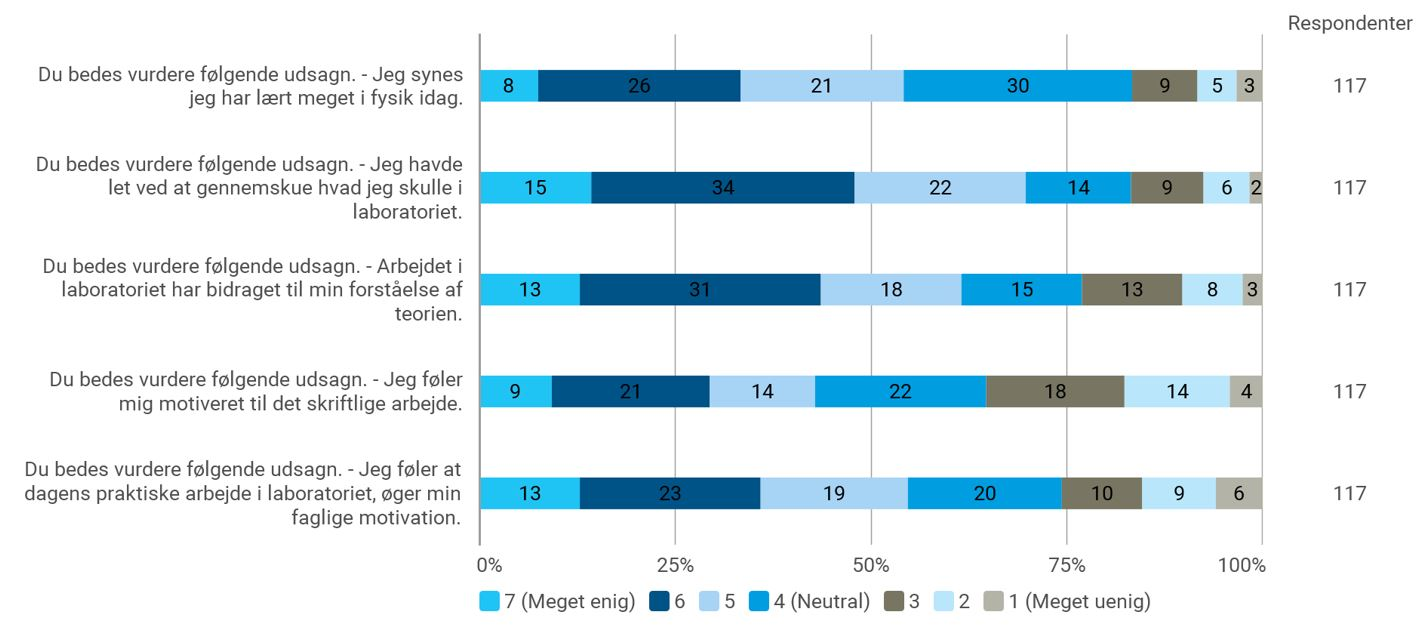
\includegraphics[width=0.9\textwidth]{Figs/Sammenlign}
	\caption{Sammenligning af de resultater som er indsamlet med spørgeskemaet.}
	\label{fig:4.1.a}
\end{figure}

Til alle fem spørgsmål i figuren udgør svarene fra neutral til meget enig i gennemsnit 66,32 \% det lader altså til baseret på dette relativt smalle datasæt at eleverne føler at de motiveres af det praktiske arbejde.

\begin{figure}[h!]
	\centering
	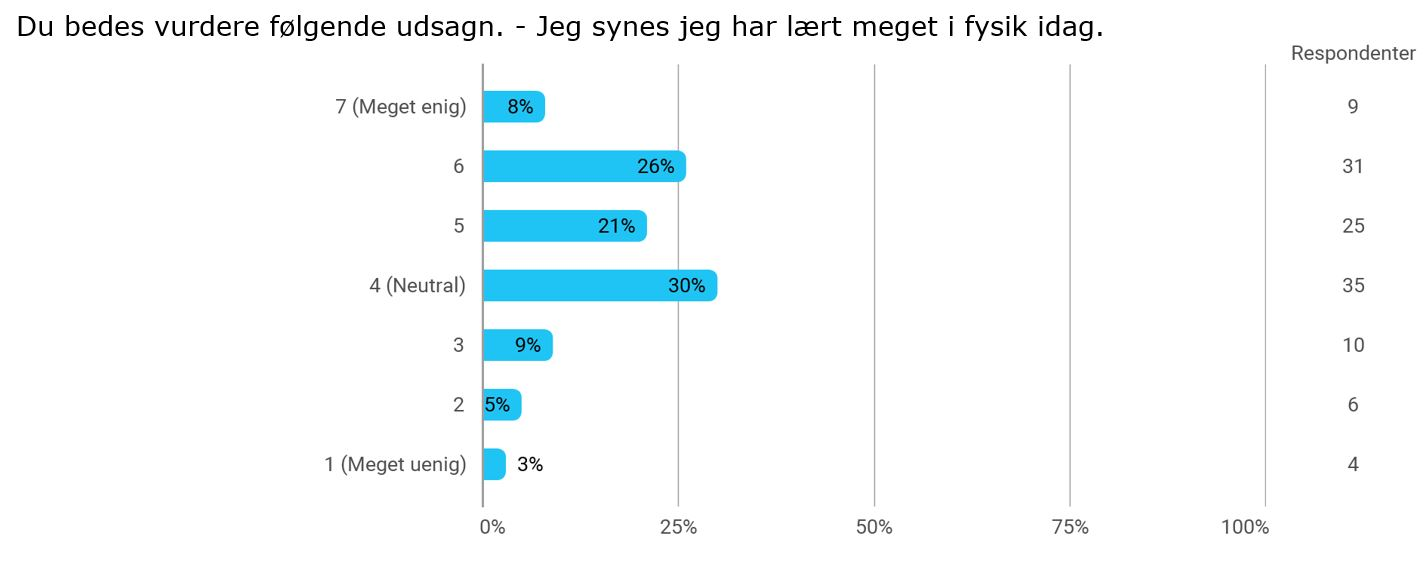
\includegraphics[width=0.9\textwidth]{Figs/Sp1}
	\caption{Spørgeskema svar fra spørgsmål 1.}
	\label{fig:4.1.b}
\end{figure}


\begin{figure}[h!]
	\centering
	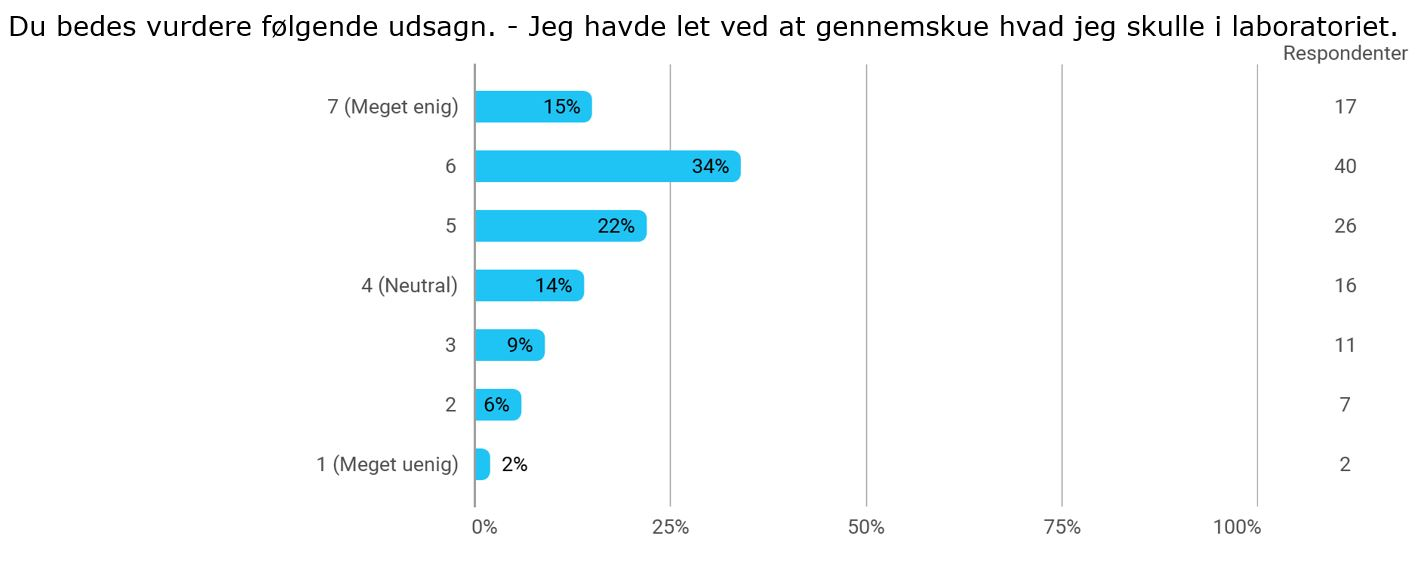
\includegraphics[width=0.9\textwidth]{Figs/Sp2}
	\caption{Spørgeskema svar fra spørgsmål 2}
	\label{fig:4.1.c}
\end{figure}

\begin{figure}[h!]
	\centering
	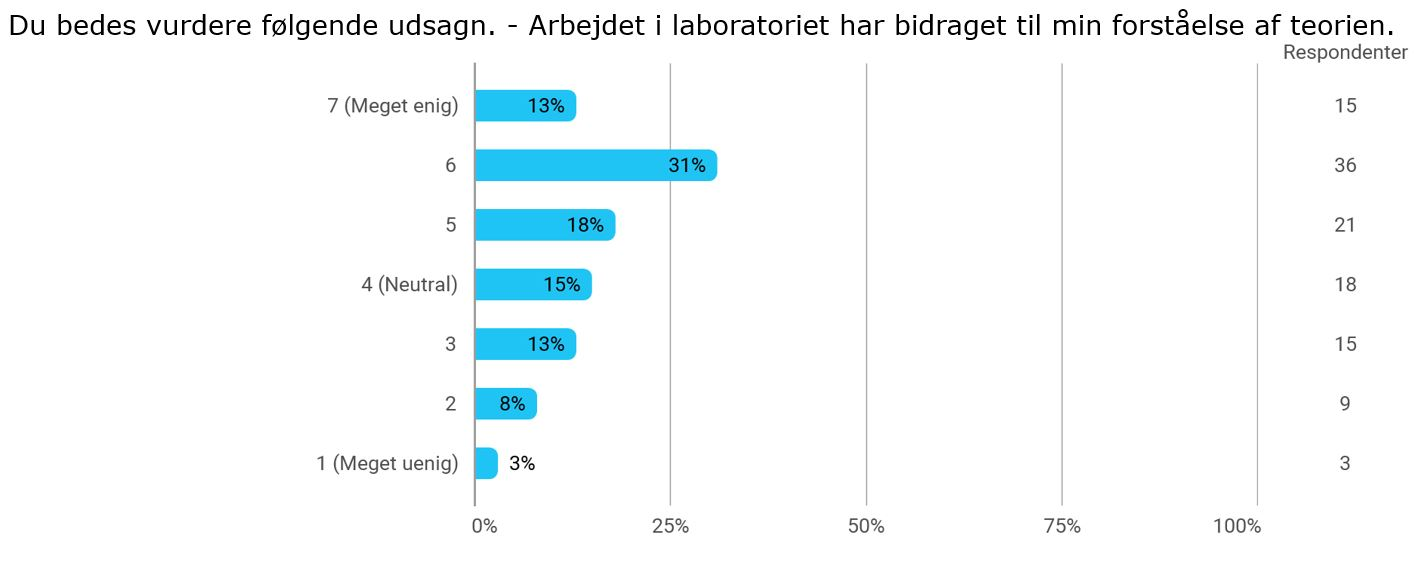
\includegraphics[width=0.9\textwidth]{Figs/Sp3}
	\caption{Spørgeskema svar fra spørgsmål 3}
	\label{fig:4.1.d}
\end{figure}

\begin{figure}[h!]
	\centering
	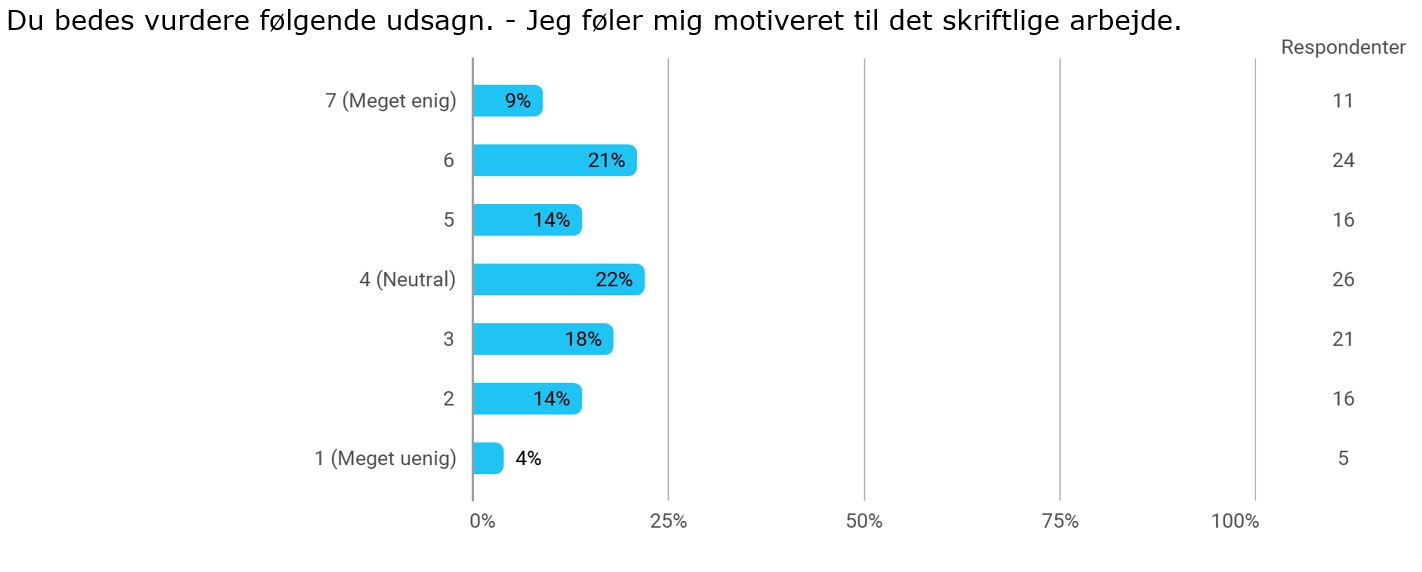
\includegraphics[width=0.9\textwidth]{Figs/Sp4}
	\caption{Spørgeskema svar fra spørgsmål 4}
	\label{fig:4.1.e}
\end{figure}

\begin{figure}[h!]
	\centering
	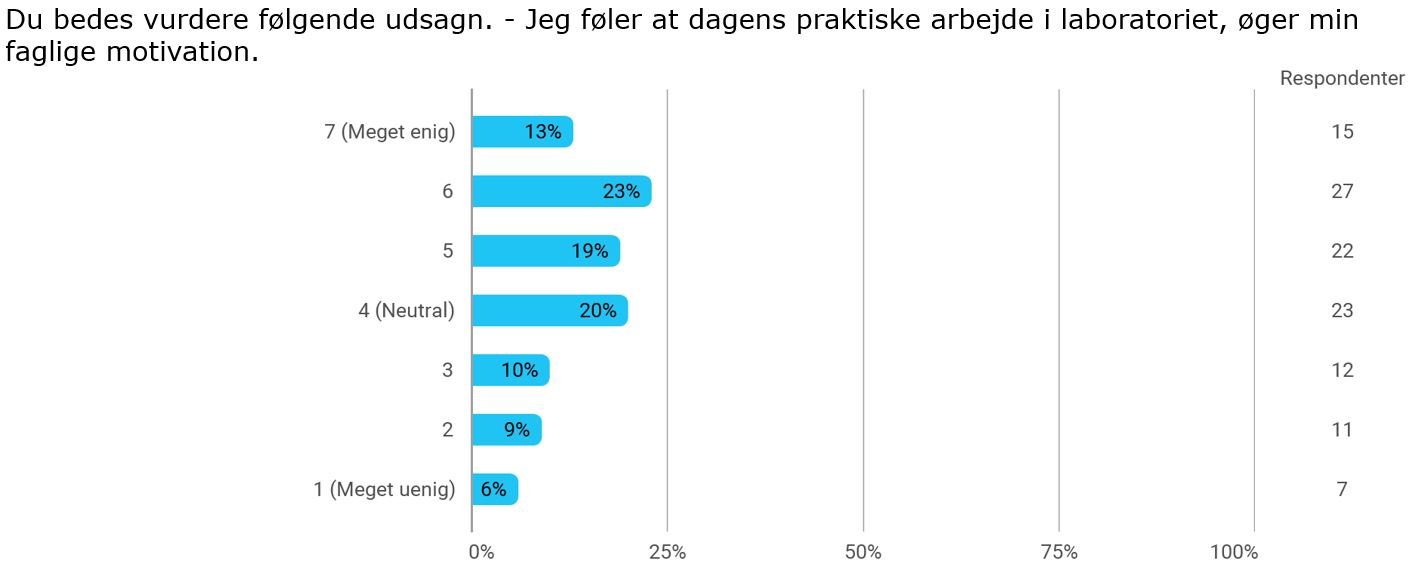
\includegraphics[width=0.9\textwidth]{Figs/Sp5}
	\caption{Spørgeskema svar fra spørgsmål 5}
	\label{fig:4.1.f}
\end{figure}
 % Analyse, fortolkning og resultater
\chapter{Diskussion og opsummering}
\label{Ch:5}

\section{Hvordan påvirkes 1.g elever af \ib{} og SWH?}
\label{sec:ibseswh}
Hvad kan der så uddrages af denne undersøgelse af elevernes motivation for det skriftlige arbejde og udviklingen af deres skriftlige kompetencer ved brug af \ib{} og SWH? Det bliver svært at uddrage noget generelt på baggrund af dette relativt lille pilotstudie på et relativt beskedent ensemble af elever. Dog kan det uddrages at eleverne ikke er helt trygge ved de frie rammer som kommer med \ib{}-metoden, det kræver tilvending for eleverne før de er helt trykke ved arbejdsformerne i \ib{}. De efterlyser mere styring, til trods herfor. Fremgår det med alt tydelighed af deres afleveringer at de har et højt udbytte af den mere frie tilgang som \ib{} giver dem. Samspillet med SWH giver en rigtig velstruktureret argumentation som indikerer et højt læringsniveau for eleverne. 

\begin{figure}[h!]
	\centering
	\usetikzlibrary{decorations.text}
	\begin{tikzpicture}
		%\draw[very thin, red!25, step=1 mm, anchor= south east] (0,0) grid (12,12);
		%\draw[thick, red!50, step=5 mm, anchor= south east] (0,0) grid (12,12);
		%\draw[very thick, red!75, step=10 mm, anchor= south east] (0,0) grid (12,12);
		
		\filldraw[very thick, draw=black, fill=red!50] (6,6) circle (5cm);
		\filldraw[very thick, draw=black, fill=white] (6,6) circle (4cm);
		\filldraw[very thick, draw=black, fill=blue!50] (6,6) circle (2.5cm);
		
		\draw[very thick] (0.5,6) -- (4.5,6) (7.5,6) -- (11.5,6) (6,0.5) -- (6, 4.5) (6,10.75) -- (6,11.5) (6,7.5) -- (6,8.75);
		
		\node at (6,6) {Tryghedszonen};
		\path [decorate, decoration= {text along path, text={Zonen for nærmeste læring}}]
		(3.75,8) arc (140:0:3cm);
		\path [decorate, decoration= {text along path, text ={Utryghedszonen}}]
		(4.75,10) arc (110:0:3.95cm);
	\end{tikzpicture}
	\caption[Vygotskys udviklingszoner]{Grafisk model af Vygotskys udviklingszoner, her inddelt i tryghedszonen hvor man kan løse de opgaver man stilles over for, zonen for nærmeste læring hvor man skal have hjælp til at løse opgaverne men hvor man gennem mestring vil blive dygtigere og sluttelig utryghedszonen hvor man mister håbet. }
	\label{fig:vyg}
\end{figure}

Eleverne oplever stor frustration over de mere frie opgaver som stilles, dette skyldes at eleverne mener at der er noget som er ``de gode'' eksperimenter og noget som er ``de dårlige'' eksperimenter. Eleverne er sikker på at der er et endeligt facit med opgaven, tanken om at der skal to streger under facit i naturfagene. Skal man være tro mod principperne i \ib{} skal eleverne selv drive eksperimentet dermed vil der aldrig blive noget egentligt facit på eksperimenterne. Omend nogle eksperimenter er mere meningsfyldte at udføre end andre. Eleverne frustreres ligeledes over hvad de betegner som dårlige data, med dette mener de data hvor de har svært ved at uddrage noget. Dette er imidlertid en pædagogisk pointe at alle data kan fortælle noget om den virkelighed der undersøges og dermed vil det pege tilbage i det oprindelige undersøgelsesspørgsmål, endvidere vil disse data med tilhørende undersøgelsesspørgsmål fortælle noget om elevernes nuværende kognitive faglige niveau.  Elevernes frustrationer her skyldes at de tvinges ud i zonen for nærmeste læring, se figur \firef{vyg}, og derved får muligheden for at udvikle sig, men det kommer med en pris. Prisen for denne udvikling er at man er nødt til at arbejde og at man gør en indstats for at udvikle sig. Eleverne vil helst som de fleste andre mennesker helst befinde sig i deres trykhedszone hvor de har helt styr på alle ting og de udfordringer de stilles overfor. Underviser man eleverne således at de ikke flyttes ud af denne zone vil man få elever som ikke udvikler sig og dermed ikke tilegner sig nye færdigheder. 

Ser man bort fra elevernes frustrationer over at de har svært ved at arbejde på denne nye og anderledes måde at tilgå viden i fysikfaget når man ikke starter med teorien men derimod med fænomenet. Så fremgår det af de undersøgte afleveringer at elevernes evner inden for faget er rykket betydeligt. Eleverne har med andre ord rykket grænsen for deres trykhedszone, således at denne er blevet udvidet. Med denne udvidelse af trykhedszonen vil også zonen for nærmeste læring også udvide sig. Denne udvikling er eleverne ikke nødvendigvis bevidste om men det står klart for underviserne som har med eleverne at gøre til daglig.

\section{Faglig motivation}
\label{sec:faglig}
Klassen 1.y har en høj grad af faglig motivation. Eleverne i klassen har aktivt valgt fysik A og matematikA  som studieretningsfag. Det er dermed svært at finde elever som er mere motiverede for faget end netop disse elever. Udfordringen her er altså hvorvidt det er muligt at dokumenterer ændringer i den faglige motivation som følge af undervisningen efter \ib-tanken med særligt fokus på SWH. Problemet her er at eleverne i klassen 1.y's svar på spørgeskemet ikke er tilgængelige som egne svar uden de øvrige 1.g elevers svar. Derved drukner eventuelle informationer om elevernes faglige motivation med fokus på det skriftlige arbejde, som følge af praktisk arbejde, i baggrunden af de øvrige svar fra 1.g'erne på Viborg Katedralskole.
Af samtalen med klassen 1.y fremgik det at de følte sig højere motiveret ved mundtligt arbejde grundet den direkte feedback og at de oplever at de lettere kan fortolke den feedback de får fra underviser og klassekammerater. Men de har mange bud på hvordan man ville kunne øge deres faglige motivation i forhold til det skriftlige arbejde. Her vil idéer som at skrive rapporterne i mindre bidder såvel som at have skrive moduler umiddelbart efter et modul med praktisk arbejde. Ligeledes vil det at dele opgaveskrivningen op i mindre bidder også give mulighed for at give eleverne noget mere mundtlig feedback på det skriftlige arbejde. 

\section{Skriftlige kompetencer}
\label{sec:skr}
Tilbage står nu hvordan det så er gået med de skriftlige kompetencer hos eleverne i 1.y kontra de skriftlige kompetencer i klassen 1.e. Det fremstår tydeligt at har eleverne ikke en veldefineret opgave så ved de ikke nøjagtig hvilke beregninger de skal foretage for at nå i mål med arbejdet hvilket gør dem utrykke.
 Det er fra analysen klart at eleverne i 1.y har udviklet sig i meget højere grad i forhold til 1.e. Hvilket stemmer fint overens med de øvrige studier inden for området. Foruden en mere fornuftig argumentation i det skriftlige arbejde ses også et mere velreflekteret skriftligt produkt hvor eleverne i 1.y afsøger mange flere mulige forklaringer på deres problemstillinger. Endvidere lader det til at eleverne i højere grad formår at forholde sig konstruktivt til eksperimenter som ikke har det forventede udfald.  % Diskussion og Opsummering
\chapter{Konklusion}
\label{Ch:6}

Med udgangspunkt i den indsamlede empiri og den gennemførte analyse af denne empiri, som danner grundlaget for dette pilot projekt, kan det konkluderes at det ikke er muligt i disse data at se nogle effekter på elevernes motivation for skriftligt arbejde. Hvilket skyldes problemer med den foreliggende empiri. Eleverne udtrykker når de bliver adspurgt at de har en meget højere lyst til at lære i forhold til det mundtlige arbejde frem for det skriftlige arbejde. Eleverens begrundelse herfor er at de føler at de har lettere ved at fortolke og afkode den feedback de får mundtligt, frem for når de modtager den på skrift. Udfordringen kan her være fastholdelse af feedbacken i forhold til at gøre den til feedforward, således at det bliver tydeligt hvad eleverne skal tage med videre, jf. slutningerne præsenteret af \citet{Hattie2015}. Eleverne giver altså idéer til hvordan man ville kunne øge den faglige motivation blandt elever i forhold til skriftlig fysik, her med fokus på skriftligt arbejde i form af rapporter og journaler. Generelt set kan det uddrages af figur \firef{4.1.a} er at eleverne generelt finder faglig motivation i det praktiske arbejde hvilket også afspejles i det indtryk de fleste fysik undervisere i det almene gymnasium påpeger, jf. \citep{Krogh2016}.

Fra analysen af fremstår det tydeligt at elev produkterne i 1.y er der en højere grad af analytisk og reflektiv tilgang til det praktiske arbejde. Der er heller ikke på samme måde berøringsangst med eksperimenter som ikke giver det forventede udfald. I klasser som ikke er undervist efter \ib{} og SWH, oplever man at eleverne frustreres over data som ikke passer med den teori de skulle eftervise, eller som slet ikke reflektere over at der er en mulig uoverensstemmelse mellem teori og data. Dette er bestemt ikke tilfældet med test klassen i denne kontekst. Det kan derfor sluttes at elevernes skriftlige kompetencer er øget betydeligt i forhold til kontrol klassen 1.e.

Sluttelig kan det konkluderes at samspillet mellem \ib{} og SWH giver mening i forhold til at udvikle elevernes kritiske rationelle sans i forhold til eksperimenter og analysen af de indsamlede eksperimentelle data. I forhold til elevernes faglige motivation kan man ud fra betragtininger af eleverne i undervisingen uddrage at \ib{} øger motivationen for det faglige arbejde og for undren over fænomener inden for fysikkens dogmæne, som beskrevet hos \citet{Dolin2014}. Det står også klart at SWH metoden understøtter netop den reflektive process i fysik faget. Udfordringerne ved at arbejde på denne metode er at det er meget tidskrævende, og i et presset pensum vil det ofstest være et sted hvor man som underviser vælger fra. \bigskip

Denne pilot undersøgelse har nogle interessante perspektiver men der er et klart behov for yderligere undersøgelser af de effekter som dette projekt indikerer der kunne være. 


\section{Perspektivering}
\label{sec:per}

En af de store udfordringer i brugen af \ib{} og SWH er at dette tager meget længere tid end at gennemfører øvelser på denne måde. Hvis blot man kan dokumentere at elevernes kompetencer udvikles mens de arbejder. Med udgangspunkt i dette pilot studie er der indicier for at elevernes skriftlige kompetencer forbedres betydeligt i forhold til den klassiske kogebogsøvelse. Der er noget der tyder på at eleverne bliver dygtigere til at gennemfører og analysere praktisk arbejde og de resultater som kommer ud af den empiri som eleverne indsamler gennem det praktiske arbejde.\bigskip


Det vil altså være nødvendigt med et yderligere studium af samspillet mellem \ib{} og SWH. Her bør man overveje en større poppulation af elever og ligeledes et bredere spektrum i forhold til studieretninger, ligeledes bør man også have et bredere udsnit af undervisere inden for fysik faget som kan indgå i projektet. Hertil kommer en kontrolgruppe som gennemfører projekt perioden men med klassiske kogebogsvejledninger.\bigskip



 % Konklusion
\chapter{Perspektivering}
\label{Ch:7}

Se \vref{sec7.1}

%\lipsum*

\section{Afsnit 1}
\label{sec:7.1}

%\lipsum* % Perspektivering

% -------- BACKMATTER ---------- %
%\backmatter
\nocite{*}
\bibliography{Bibliografi/SWH}

\appendix

\chapter{Science Writing Heuristic eller at skrive for at lære}
 \label{app:A}
 
 Hvis du spørger dine klassekammerater eller din underviser efter en definition på begrebet \emph{undersøgelse}, vil du formentlige få ligeså mange forskellige unikke definitioner som antallet af personer du har spurgt. Dette skyldes at \emph{undersøgelse} kan have mange forskellige meninger uafhængigt af personen der spørges. I denne laboratorie manual, har vi valgt følgende forståelse af begrebet \emph{undersøgelse} som midlerne til at gennemføre videnskab. For at hjælpe dig til at tænke hele vejen igennem den videnskabelige process har vi struktureret denne manual med overskrifter som er draget ud fra pricippet science writing heuristic (SWH).
 
SWH er en velbeskrevet metode til at styre undersøgelsesbaserede oplevelser, og den er designet til at opfordre til konstruktion af konceptuel viden i faget. Metoden er også baseret på sammenhængen mellem spørgsmål, evidens og påstande. Den oprindelige udgave af science writing heuristic inkluderede følgende processer som du som elev skal igennem.
 
 \begin{enumerate}
 	\item Første spørgmål til undersøgelsen\vspace{-15pt}
 	\item Test\vspace{-15pt}
 	\item Observationer\vspace{-15pt}
 	\item Påstande\vspace{-15pt}
 	\item Evidens\vspace{-15pt}
 	\item Læsning\vspace{-15pt}
 	\item Refleksion\vspace{-15pt}
 	\item Skrive fase
\end{enumerate}

Ovenstående otte kategorier er blevet tilpasset arbejdet med undersøgelser, således at de nu er følgende overskrifter. Under hver af overskrifterne finder du en kort instruks, som forholder sig til den undersøgelse som relaterer sig til overskrifter. Overskrifterne kobler også til de faglige mål i fysik faget.

\section{Stil spørgsmål}
\label{sec:SS}
Enhver videnskabelig undersøgelse begynder normalvis med en undren der kan formuleres som et spørgsmål. Dette spørgsmål skal så besvares gennem eksperimenter hvor man indsamler data. Fra tid til anden er dette spørgsmål givet på forhånd, mends det andre gange vil være dig der skal stille spørgsmålet sammen med din laboratorie gruppe.

\section{Forberedelse af undersøgelse}
 \label{sec:FaU}
 Før du kan påbegynde dit praktiske arbejde, er det vigtigt at der er en klar plan for hvordan du vil indsamle dine data, som skal danne grundlaget for din evidens senere. Dette inkluderer også at indetificere hvilke data der skal indsamles og hvilke skridt der skal følges i laboratoriet. I nogle tilfælde vil, en fuldstændig eller delvis procedure være indkluderet i vejledningen til undersøgelsen. I de fleste tilfælde skal du dog udlede dele af eller hele proceduren sammen med din laboratoriegruppe. Uanset om proceduren er givet eller du skal lave den, skal du studere den nøje forud for det praktiske arbejde. Du er også nødt til at fremstille et system til at nedfælde observationer og målinger fra undersøgelsen - fx en tabel eller et skema enten på papir eller i excel.
 
 \section{Lav forudsigelser}
 \label{sec:LF}
 I langt de fleste undersøgelser, bør du prøve at forudsige hvad du forventer der sker når du indsamler evidens. Disse forudsigelser skal være baseret på dine egne erfaringer og vil på ingen måde blive vurderet for deres korrekthed, men du kan med fordel reflektere over dem efter at have gennemført det praktiske arbejde - passer din forståelse med det eksperimentet viser?
 
 \section{Indsamling af empiri}
 \label{sec:IaE}
 Hjørnestenen i enhver undersøgelse er indsamlingen af empiri som danner grundlaget for den evidens som senere skal underbygge dine påstande. Når du indsamler empiri skal du være opmærksom på at få alle tal noteret korrekt i det skema/den tabel du har lavet til formålet. Endvidere skal du sørge for at notere alt hvad du observerer. Dette kan indeholde retninger, skridt foretaget i undersøgelsen, eller en guide til indsamling af empiri og øvrige observationer.
 
 \section{Analyse af empiri}
 \label{sec:AaE}
 Den indsamlede empiri vil i de fleste tilfælde kræve at du foretager yderligere behandling af data før du kan svarer på dit oprindelige spørgsmål fra afsnit \vref{sec:SS}. Inden du går i krig med din empiri bør du kigge på dine data og se om der er noget som springer i øjnene fx punkter som afviger klart fra de øvrige eller generelle tendenser som fremstår klart fra den indsamlede empiri. Herefter bør du foretage de nødvendige beregninger eller en grafisk analyse af den indsamlede empiri. Her vil det være fint at vise et regne eksempel med et eller to datapunkter. Resultatet af din analyse er den evidens som skal underbygge de påstande du har fremhævet baseret på den indsamlede empiri.
 
 \section{Fortolkning af evidens}
\label{sec:FaE}
Når du har analyseret din empiri, og nu har noget evidens, bør du altid spørge dig selv, ``Hvad betyder denne evidens?'' For at kunne besvarer dette spørgmål, er du nødt til at foreslå forklaringer/påstande på de videnskabelige fænomener. Spørgsmål i dette afsnit er designet for at hjælpe dig med at tænke over de konsekvenser som evidensen medfører og at rette eller korrigere denne til et meningsfuldt formål med undersøgelsen.

\section{Fremstilling af påstande}
\label{sec:FaP}
Når du er i mål med en analyse og en fortolkning af din empiri, og du har fremsat et svar på dit indledende spørgsmål. Bør du omformulere dette til en videnskabelig påstand. En sådan påstand skal altid kunne underbygges med evidensen fra undersøgelsen. Når du har fremstillet påstande bør du kigge i litteraturen for at underbygge dem med andres viden.

\section{Reflektion over undersøgelsen}
\label{sec:RoU}
Den afsluttende opgave i de fleste undersøgelser er at reflektere over hvad der blev gjort, overvej hvordan din forståelse har udviklet sog, og anvend din nye viden på andre lignende situationer.

\section{Noter}
Det er mit håb at denne manual vil kunne hjælpe dig i forarbejdet til dit skriftlige arbejde med undersøgelser, og at den ligeledes vil hjælpe dig til at blive en bedre videnskabsmand. Denne instruktion er sammensat af viden fra \citep{Hand2004, Greenbowe2005, Krogh2016}


\chapter{Nyttevirkning af elkedel og kaffemaskine}
\label{app:B}

\section{Formål}
Formålet med øvelsen er at bestemme den nyttevirkning, hvormed nogle almindelige elektriske apparater omsætter elektrisk energi. I dette tilfælde undersøges en elkedel og en kaffemaskine.

\section{Teori}
Når man benytter et elektrisk apparat, vil en del af den elektriske energi, der omsættes, gå til spilde. Opvarmer man f.eks. vand i en kedel, bruges en del af den tilførte elektriske energi til opvarmning af kedlen og omgivelserne.
Ved nyttevirkningen eller effektiviteten (betegnes med det græske bogstav $\eta$ (eta)) af et apparat forstår man forholdet mellem den udnyttede energi og den tilførte energi angivet i procent:
\begin{equation*}
	\eta = \frac{\Delta E_{\mathrm{nyt}}}{\Delta E_\mathrm{til}}\cdot 100 \%
\end{equation*}
$\Delta E_\mathrm{til}$ er i denne øvelse den elektriske energi, som et apparat omsætter. Derfor udregner man $\Delta E_\mathrm{til}$ ved hjælp af formlen:
\begin{equation*}
\Delta E_\mathrm{til} = P\cdot \Delta t
 \end{equation*}
hvor $P$ er apparatets effektforbrug og $\Delta t$ er den tid, hvor apparatet er tændt.
$\Delta E_{\mathrm{nyt}}$ er den energi, som udnyttes til opvarmning af vandet. Når vi har en mængde vand med massen $m$, kan denne energi beregnes ved hjælp af formlen:
\begin{equation*}
\Delta E_{\mathrm{nyt}} = m\cdot c\cdot \Delta T = m\cdot c\cdot (T_{2} – T_{1})
\end{equation*}
hvor $c$ er den specifikke varmekapacitet (varmefylde) for vand. $c$ har værdien \mbox{4180 $\joule\per(\kilo\gram\cdot\celsius)$}.
$T_1$ og $T_2$ er vandets begyndelses- og sluttemperatur.

Bemærk, at vi i denne øvelse bruger symbolet $t$ for tid og $T$ for temperatur.

\section{Apparatur}
Elkedel, kaffemaskine, stopur, måleglas, termometer, effektmåler, vægt.

\section{Opstilling}
Tegn selv opstillingen eller tag et billede af den.

\section{Udførelse}
\begin{itemize}
	\item[1)] {\bfseries Elkeden:}
	Der afmåles ca. 1,0 kg vand i elkedlen. Effektmåleren sættes i stikkontakten, og elkedlen kobles til effektmåleren. Vandets begyndelsestemperatur $T_{1}$ aflæses. Elkedlen og stopuret tændes samtidig. På effektmåleren aflæses den effekt, hvormed der omsættes elektrisk energi. Når vandet koger, antager i at sluttemperaturen $T_2$ er 100 \celsius, hvilket i noterer i jeres skema. Den forløbne tid $\Delta t$ noteres.
	\item[2)] {\bfseries Kaffemaskienen:}
	Målingerne forløber som ved elkedlen. Vandets sluttemperatur er temperaturen af det vand, der er løbet ned i kaffemaskinen. Tidtagningen slutter, når alt vandet er løbet igennem og i aflæser sluttemperaturen $T_2$. På effektmåleren aflæses den effekt, hvormed der omsættes elektrisk energi.
\end{itemize}

\section{Måleresultater}
\begin{table}
\centering
\caption{pris/kWh = \hspace{5cm} $c$ =}
\label{tbl:data.forsøg1}
\begin{tabular}{ @{ } p{3cm}  p{3cm}  p{3cm} @{ } }
	\toprule[2pt]
			&	Elkedel	&	Kaffemaskine	\\
	\midrule[1.2pt]
	$m (\kilo\gram)$					&			&				\\
	$T_{1} (\celsius)$					&			&				\\
	$T_{2} (\celsius)$					&			&				\\
	$\Delta T (\celsius)$					&			&				\\
	$\Delta E_{\mathrm{nyt}} (\joule)$		&			&				\\
	$P (\watt)$						&			&				\\
	$\Delta t (\second)$					&			&				\\
	$\Delta E_{\mathrm{til}} (\joule)$		&			&				\\
	$\eta (\%)$						&			&				\\
	$\Delta E_{\mathrm{til}} (\kilo\watt\hour)$	&			&				\\
	Pris (kroner)						&			&				\\
	\bottomrule[2pt]
\end{tabular}
\end{table}

\section{Databehandling}
\begin{enumerate}
	\item De tomme rubrikker i skemaet udfyldes og medtages i rapporten. Og der vises eksempler på udregninger for elkedlen i de efterfølgende spørgsmål.
	\item Udregning af temperaturtilvæksten $\Delta T$.
	\item Udregning af den udnyttede energi  $\Delta E_{\mathrm{nyt}}$
	\item Udregning af den tilførte energi $\Delta E_{\mathrm{til}}$
	\item Udregning af nyttevirkningen $\eta$
	\item Udregning af den tilførte energi $\Delta E_{\mathrm{til}}$ i \kilo\watt\hour
	\item Udregning af prisen for at opvarme vandet.
\end{enumerate}
Du må naturligvis gerne bruge kaffemaskinen i stedet for elkedlen til at vise eks. på udregninger. Du skal så blot angive det.

\section{Diskussion}
Diskuter resultaterne. Man kan f.eks. komme ind på følgende spørgsmål:
\begin{itemize}
	\item Hvilket af de to apparater udnytter den elektriske energi bedst?
	\item Hvilke fordele og ulemper kan man nævne ved hvert af de to apparater, når de bruges til at lave \'en liter kaffe?
	\item Hvad er prisen for den elektriske energi, der omsættes, når man laver én liter kaffe henholdsvis på kaffemaskinen og ved hjælp af elkedlen?
\end{itemize}

 \section{konklusion}

\chapter{Undersøgelse af diffraktion}
\label{app:C}
Hvis man betragter den problemstilling som eleverne i gruppen med elev 4 havde under forsøget med fænomenet diffraktion af laserlys. Så kan det diskuteres om eleverne har de fornødne færdigheder til at kunne foretage en fyldestgørende analyse af problemet i forhold til at frembringe evidens og rygdæknig for en påstand. 
Udgangspunktet er følgende eksperimentelle opstilling se figur \firef{ops.app}
\begin{figure}[h!]
	\centering
	\begin{tikzpicture}
		%\draw[very thin, blue!25, step=1mm, anchor=south east] (0,0) grid (12,6);
		%\draw[blue!50, step=5mm, anchor=south east] (0,0) grid (12,6);
		%\draw[thick, blue!75, step=10mm, anchor=south east] (0,0) grid (12,6);
		
		\draw[thick, black] (7,2.5) arc (0:12:1.9cm);
		\draw[thick, black] (7.5,2.5) arc (0:23:2.4cm);
		
		\filldraw[fill=white,draw=black, thick] (0,2.25) -- (2,2.25) -- (2,2.75) -- (0,2.75) -- cycle;
		\draw[very thick, red] (2,2.5) -- (12,2.5) node[black,right] {$n = 0$};
		\draw[very thick, fill=red,draw=red] (12,2.5) circle (1mm);
		
		\draw[very thick, red] (5.1,2.5) -- (12,4) node[black,right] {$n = 1$};
		\draw[very thick, fill=red,draw=red] (12,4) circle (1mm);
		
		\draw[very thick, red] (5.1,2.5) -- (12,5.5) node[black,right] {$n = 2$};
		\draw[very thick, fill=red,draw=red] (12,5.5) circle (1mm);
		
		\draw[very thick, draw=black,fill=black] (4.9,1) rectangle (5.1,4) node[above] {Gitter};
		
		\node at (6.75,2.75) {$\theta_1$};
		\node at (7.75,2.75) {$\theta_2$};
		\node at (1,2.5) {Laser};
		\draw[very thick, black, <-] (5.1,1.5) -- (8,1.5);
		\draw[very thick, black, ->] (9,1.5) -- (12,1.5);
		\node at (8.5,1.5) {$L$};
		\draw[very thick, black, <-] (12,2.6) -- (12,3);
		\draw[very thick, black, ->] (12,3.5) -- (12,3.9);
		\node at (12,3.24) {$S_1$};
	\end {tikzpicture}
	\caption{Forsøgsopstillingen til eksperimenterne som eleverne har udført dem.}
	\label{fig:ops.app}
\end{figure}

Her får eleverne brug for at anvende en tangensrelation til at bestemme afbøjningsvinklen $\theta_n$ til den $n$'te orden. 
\begin{equation}
	\theta_n = \tan^{-1}\left(\frac{S_n}{L}\right)
\end{equation}
her er $S_n$ afstanden mellem 0'te og $n$'te orden i interferensmønstret mens $L$ er afstanden mellem gitteret og målepunktet som vist på figur \firef{ops.app}. Denne værdi for vinklen indsættes på vinklens plads i gitterligningen.
\begin{equation}
	d\cdot\sin\theta_n = n\cdot \lambda
\end{equation}
hvor $d$ er gitterkonstanten, $n$ er ordensnummeret dvs et positivt heltal og $\lambda$ er laserens bølgelængde. Nu indsættes udtrykket for afbøjningsvinklen $\theta_n$ i ligningen herover of der isoleres for afstanden mellem ordenerne herved finder man følgende udtryk:
\begin{equation}
	S_n = \tan\left(\sin^{-1}\left(\frac{n\cdot\lambda}{d}\right)\right)\cdot L
\end{equation}
Modelleres dette udtryk i et matematik program med passende valg af $n$, $d$, $\lambda$ og $L$ kan man få figur \firef{eviden.app}. 
\begin{figure}[h!]
	\centering
	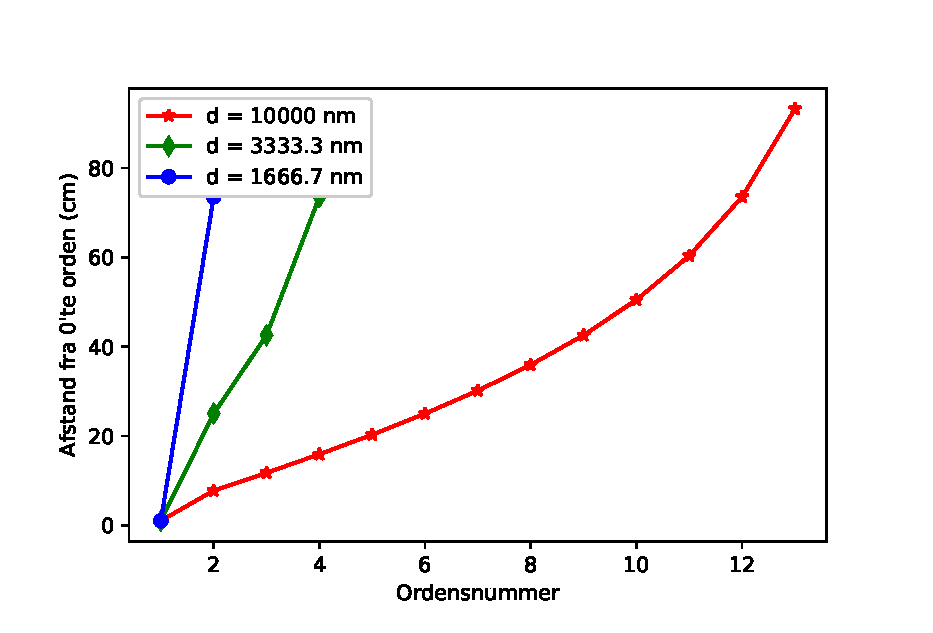
\includegraphics[width=\textwidth]{Figs/test}
	\caption{Her ses en teoretisk modelleret udgave af figur \firef{evidens.jacob} som gruppen med elev 4 frambragte eksperiementelt på baggrund af de data de havde til rådighed.}
	\label{fig:eviden.app}
\end{figure}

Her illusrerer den blå linje et gitter med 600 linjer pr mm, den grønne et gitter med 300 linjer pr mm mens den røde viser et gitter med 100 linjer pr mm. Heraf ses det at gruppen med elev 4 faktisk har ramt den overordnede trent ret godt, omend deres afstande er temmelig meget for små. % Appendix


\end{document}